
% Definieren der Dokumentklasse
\documentclass[ngerman, 11pt]{article}

% T1 Font Encoding: Sonderzeichen ä,ü,ö,... als eigene Symbole
\usepackage[T1]{fontenc}

% UTF-8 Kodierung
\usepackage[utf8]{inputenc}

% Sprache Zeichensatz Deutsch
\usepackage[ngerman]{babel}

% Nutzen Mathematischer Symbole
\usepackage{amsmath}

% Nutzen weiterer Sonderzeichen
\usepackage{amssymb}

% Schriftart: helvet als Arial-Klon
\usepackage{helvet}
\renewcommand{\familydefault}{\sfdefault}

% Anpassen des Zeilenabstandes
\usepackage[singlespacing]{setspace}
\setstretch{1.454545454545455}% Faktor: 16pt/11pt = 1.454545454545455

% Rückung neuer Absätze
\setlength\parindent{0pt}

% Einbinden von Grafiken
\usepackage{graphicx}
\graphicspath{{../Karten}{.}}

% Positionieren von Grafiken
\usepackage[export]{adjustbox}

% Definieren von Farben
\usepackage[table]{xcolor}% table Option für die Farbgestaltung von Tabellen
\definecolor{imreg}{RGB}{39, 89, 165}
\definecolor{urlcol}{RGB}{0, 0, 238}

% Erstellen von Verlinkungen und Pfaddarstellungen
\usepackage[obeyspaces]{url}
\usepackage{hyperref}
\hypersetup{
	breaklinks,
	colorlinks,
	linkcolor=black,
	urlcolor=urlcol
}

% Zuschneiden der Seite
\usepackage[paper=a4paper, top=40mm, bottom=27mm, left=20mm, right=20mm, headheight=61pt]{geometry}


\usepackage{pdflscape}

% Abstand der Bildüberschrift zum Bild
\setlength{\belowcaptionskip}{15pt}

% Nutzen und formattieren der Subfigure Umgebung
\usepackage{subcaption}
\captionsetup[subfigure]{labelformat=empty}


% Definieren von Kopf- und Fußzeile
\usepackage{fancyhdr}
\pagestyle{fancy}
\renewcommand{\headrulewidth}{1.5pt}
\let\oldheadrule\headrule\renewcommand{\headrule}{\color{imreg}\oldheadrule}
\renewcommand{\footrulewidth}{1.5pt}
\let\oldfootrule\footrule\renewcommand{\footrule}{\color{imreg}\oldfootrule}
\fancyhead[L]{\nouppercase \leftmark}
\fancyhead[C]{}
\fancyhead[R]{
\includegraphics[height=20mm]{imreg}}
\fancyfoot[L]{\color{black} Stand: \today}
\fancyfoot[C]{}
\fancyfoot[R]{\color{black} \thepage}



% Formatierung von Überschriften
\usepackage{titlesec}
% Hauptüberschriften
\titleformat{\section}
[block]% shape
{\color{imreg} \Large}% format
{\textbf{\thesection.}}% label
{11pt}% horizontal separation
{\textbf}% before-code
[]% after-code
% Hauptüberschriften
\titleformat{\subsection}
[block]% shape
{\color{imreg} \large}% format
{\textbf{\thesubsection.}}% label
{11pt}% horizontal separation
{\textbf}% before-code
[]% after-code
% Abstandsregel Hauptüberschriften
\titlespacing{\section}
{0pt}% left
{0pt}% before
{0pt}% after
\titlespacing{\subsection}
{0pt}% left
{0pt}% before
{0pt}% after


% Bild-, Tabellen- & Kartenüberschriften
\usepackage[figurename=Abb.]{caption}
\DeclareCaptionFormat{imregCaption}{\normalsize \color{imreg} \textbf{#1#2#3}}
\captionsetup{format=imregCaption, justification=centering, singlelinecheck=false}
\setlength{\abovecaptionskip}{0pt}
\setlength{\belowcaptionskip}{0pt}


% Formatieren der Listendarstellung
\usepackage{tocloft}
\renewcommand{\cftdot}{\ensuremath{}}
\renewcommand\cfttoctitlefont{\Large \bfseries \color{imreg}}
\renewcommand{\cftloftitlefont}{\Large \bfseries \color{imreg}}
\renewcommand{\cftlottitlefont}{\Large \bfseries \color{imreg}}
% Abbildungsverzeichnis
\renewcommand{\cftfigpresnum}{Abb. }% Präfix
\settowidth{\cftfignumwidth}{Abb. xx\quad}% Abstand bis Name
\setlength\cftfigindent{0pt}% Rückung
% Tabellenverzeichnis
\renewcommand{\cfttabpresnum}{Tabelle }
\settowidth{\cfttabnumwidth}{Tabelle xx\quad}
\setlength\cfttabindent{0pt}
% Zählfunktion für Karten
\newcommand{\listmapname}{Kartenverzeichnis}
\newlistof
{maps}% Funktionsname
{caption}% Platzhalter
{\Large \color{imreg} \listmapname}% Name
% Zählfunktion für Karten
\newcommand{\maps}[1]{%
	\refstepcounter{maps}
	\par\noindent \textbf{\large \color{imreg} Karte \themaps: #1}
	\addcontentsline{caption}{maps}{\normalsize Karte \themaps\quad\protect#1}\par}


% Befehl zum Erstellen einer Leerseite
\newcommand*\emptypage{\newpage\null\thispagestyle{empty}\newpage}

% Befehl zum Einbinden einer Karte
\newcommand{\karte}[3]{
	\makebox[\linewidth][c]{
		\begin{subfigure}{0.61\textwidth}
			\centering
			\caption{\\#2}
			\includegraphics[width=\textwidth, height=172mm, center]{#1} 
		\end{subfigure}
		\begin{subfigure}{0.61\textwidth}
			\centering
			\caption{\\#3}
			\includegraphics[width=\textwidth, height=172mm, center]{#1_Delta}
		\end{subfigure}
	}
}



% Informationen für das Deckblatt
\title{M+E Osteuropaatlas}
\author{Simon Gräfe}


\usepackage{lipsum}



\begin{document}

	\tableofcontents
	\listoffigures
	\listofmaps
	
	\emptypage
	\include{Kapitel/Wertschöpfung}
	\emptypage
	%!TEX root = ../Osteuropaatlas.tex

\section{Wirtschaftliche Strukturdaten}


\setcounter{figure}{1}
\begin{figure}[!h]
	\addcontentsline{toc}{subsection}{IMD Wirtschaftsleistungsranking}
	\caption{IMD Wirtschaftsleistungsranking}
	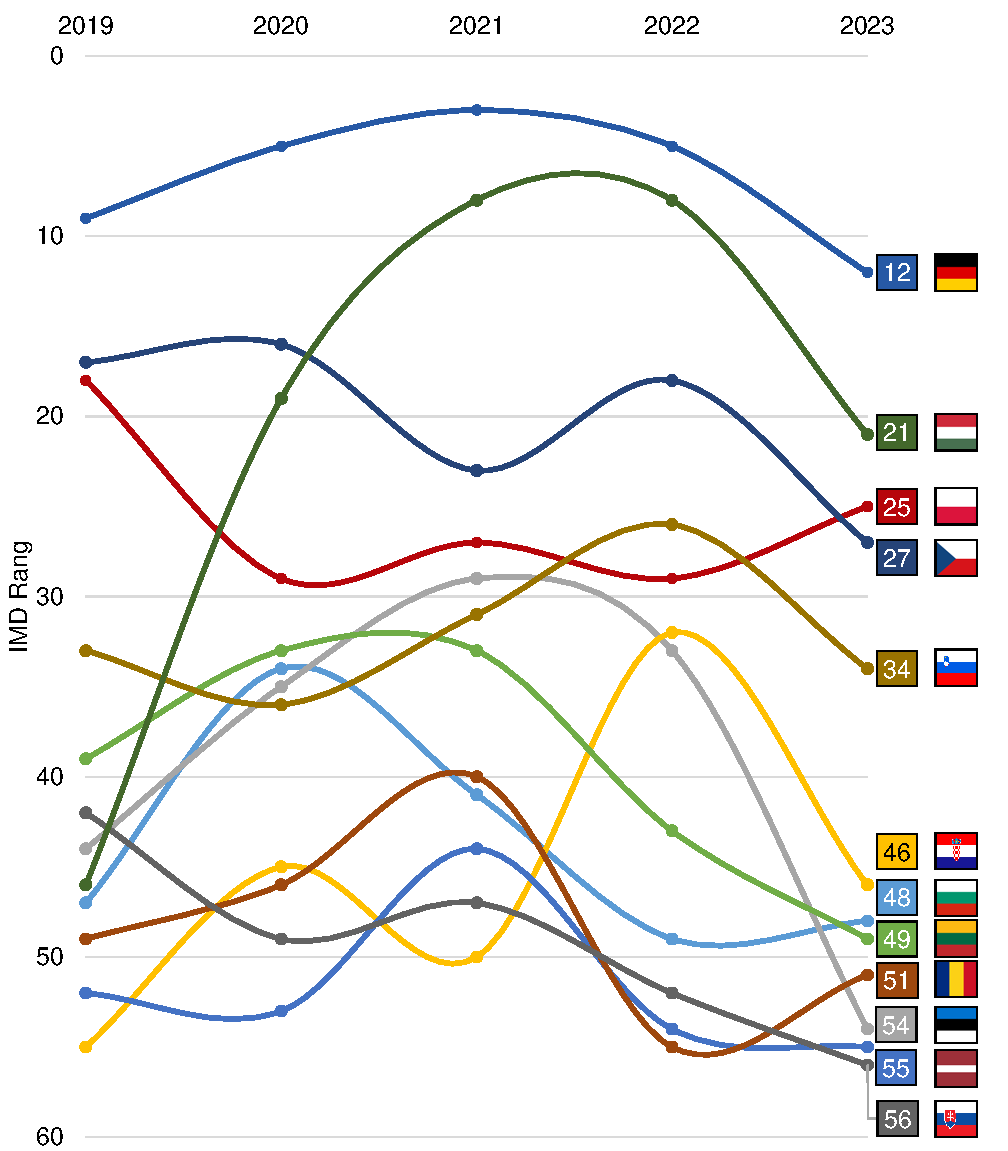
\includegraphics[width = \textwidth, height = 19.5cm]{IMD_Ranking}
	\begin{spacing}{1} \scriptsize
		\vspace{2mm}
		Anm.: IMD Economic Performance Ranking; Stand 2023\\
		Quelle: IMD World Competitiveness Center (2024); Dar. imreg (2024) \end{spacing}
\end{figure}


\begin{figure}[p]
	\addcontentsline{toc}{subsection}{Arbeitsstunden}
	{\centering \maps{Arbeitsstunden}}
	\label{map:stundengeleistet}
	\karte{Arbeitsstunden_geleistet}{2020}{Veränderung 2015 bis 2020}
	\begin{spacing}{1} \scriptsize
		Anm.: Jährliche Summe geleisteter Arbeitsstunden unabhängig von Bezahlung; Stand 2020\\
		Quelle: Eurostat (2024); Ber. \& Dar. imreg (2024) \end{spacing}
\end{figure}


\begin{figure}[p]
	\addcontentsline{toc}{subsection}{Arbeitsstunden je Erwerbstätigen}
	{\centering \maps{Arbeitsstunden je Erwerbstätigen}}
	\label{map:stundengeleistetprokopf}
	\karte{Arbeitsstunden_proErwerbstaetigen}{2020}{Veränderung 2015 bis 2020}
	\begin{spacing}{1} \scriptsize
		Anm.: Jährliche Summe geleisteter Arbeitsstunden unabhängig von Bezahlung; Stand 2020\\
		Quelle: Eurostat (2024); Ber. \& Dar. imreg (2024) \end{spacing}
\end{figure}


\begin{figure}[p]
	\addcontentsline{toc}{subsection}{Arbeitnehmerentgelt}
	{\centering \maps{Arbeitnehmerentgelt}}
	\label{map:entgelt}
	\karte{Arbeitnehmerentgelt}{2020}{Veränderung 2015 bis 2020}
	\begin{spacing}{1} \scriptsize
		Anm.: Jährliche Entgeltsumme; Stand 2020\\
		Quelle: Eurostat (2024); Ber. \& Dar. imreg (2024) \end{spacing}
\end{figure}


\begin{figure}[p]
	\addcontentsline{toc}{subsection}{Arbeitnehmerentgelt je Arbeitnehmer}
	{\centering \maps{Arbeitnehmerentgelt je Arbeitnehmer}}
	\label{map:entgeltprokopf}
	\karte{Entgelt_proKopf}{2020}{Veränderung 2015 bis 2020}
	\begin{spacing}{1} \scriptsize
		Anm.: Jährliche Entgeltsumme; Stand 2020\\
		Quelle: Eurostat (2024); Ber. \& Dar. imreg (2024) 
	\end{spacing}
\end{figure}


\begin{figure}[p]
	\addcontentsline{toc}{subsection}{Arbeitnehmerentgelt je Arbeitsstunde}
	{\centering \maps{Arbeitnehmerentgelt je Arbeitsstunde}}
	\label{map:entgeltprostunde}
	\karte{Entgelt_proH}{2020}{Veränderung 2015 bis 2020}
	\begin{spacing}{1} \scriptsize
		Anm.: Jährliche Entgeltsumme; Stand 2020\\
		Quelle: Eurostat (2024); Ber. \& Dar. imreg (2024) 
	\end{spacing}
\end{figure}


\begin{figure}[p]
	\addcontentsline{toc}{subsection}{Arbeitproduktivität je Erwerbestätigen (nominal)}
	{\centering \maps{Arbeitproduktivität je Erwerbestätigen (nominal)}}
	\label{map:prodprokopfnom}
	\karte{Arbeitsproduktivitaet_proErwerbstaetigen_nom}{2020}{Veränderung 2015 bis 2020}
	\begin{spacing}{1} \scriptsize
		Anm.: Jährlicher nominaler Produktionswert je Erwerbstätigen; Stand 2020\\
		Quelle: Eurostat (2024); Ber. \& Dar. imreg (2024) 
	\end{spacing}
\end{figure}


\begin{figure}[p]
	\addcontentsline{toc}{subsection}{Arbeitproduktivität je Arbeitsstunde (nominal)}
	{\centering \maps{Arbeitproduktivität je Arbeitsstunde (nominal)}}
	\label{map:prodprostundenom}
	\karte{Arbeitsproduktivitaet_proH_nom}{2020}{Veränderung 2015 bis 2020}
	\begin{spacing}{1} \scriptsize
		Anm.: Jährlicher nominaler Produktionswert je Arbeitsstunde; Stand 2020\\
		Quelle: Eurostat (2024); Ber. \& Dar. imreg (2024) 
	\end{spacing}
\end{figure}


\begin{figure}[p]
	\addcontentsline{toc}{subsection}{Entwicklung Arbeitsproduktivität (real)}
	{\centering \maps{Entwicklung Arbeitsproduktivität (real)}}
	\label{map:bipvol}
	\makebox[\linewidth][c]{
		\begin{subfigure}{0.61\textwidth}
			\centering
			\caption{Arbeitproduktivität je Erwerbestätigen (real)\\Veränderung 2015 bis 2020}
			\includegraphics[width=\textwidth, height=172mm, center]{Arbeitsproduktivitaet_proErwerbstaetigen_real_Delta} 
		\end{subfigure}
		\begin{subfigure}{0.61\textwidth}
			\centering
			\caption{Arbeitproduktivität je Arbeitsstunde (real)\\Veränderung 2015 bis 2020}
			\includegraphics[width=\textwidth, height=172mm, center]{Arbeitsproduktivitaet_proH_real_Delta}
		\end{subfigure}
	}
	\begin{spacing}{1} \scriptsize
		Anm.: Jährlicher nominaler Produktionswert je Erwerbestätigen/Arbeitsstunde Stand 2020\\
		Quelle: Eurostat (2024); Ber. \& Dar. imreg (2024) \end{spacing}
\end{figure}


\begin{figure}[p]
	\addcontentsline{toc}{subsection}{Anlageninvestitionen}
	{\centering \maps{Anlageninvestitionen}}
	\label{map:invest}
	\karte{Anlageninvestition}{2020}{Veränderung 2015 bis 2020}
	\begin{spacing}{1} \scriptsize
		Anm.: Anlageninvestitionen; Stand 2020\\
		Quelle: Eurostat (2024); Ber. \& Dar. imreg (2024) 
	\end{spacing}
\end{figure}


\begin{figure}[p]
	\addcontentsline{toc}{subsection}{Anzahl Unternehmen im Verarbeitenden Gewerbe}
	{\centering \maps{Anzahl Unternehmen im Verarbeitenden Gewerbe}}
	\label{map:unternehmenvg}
	\karte{StrukturVG_UntZahl}{2020}{Veränderung 2015 bis 2020}
	\begin{spacing}{1} \scriptsize
		Anm.: Stand 2020\\
		Quelle: Eurostat (2024); Ber. \& Dar. imreg (2024) 
	\end{spacing}
\end{figure}


\begin{figure}[p]
	\addcontentsline{toc}{subsection}{Anzahl Beschäftigter im Verarbeitenden Gewerbe}
	{\centering \maps{Anzahl Beschäftigter im Verarbeitenden Gewerbe}}
	\label{map:beschvg}
	\karte{StrukturVG_BeschZahl}{2020}{Veränderung 2015 bis 2020}
	\begin{spacing}{1} \scriptsize
		Anm.: Stand 2020\\
		Quelle: Eurostat (2024); Ber. \& Dar. imreg (2024) 
	\end{spacing}
\end{figure}


\begin{figure}[p]
	\addcontentsline{toc}{subsection}{Anteil Beschäftigter im Verarbeitenden Gewerbe an allen Beschäftigten}
	{\centering \maps{Anteil Beschäftigter im Verarbeitenden Gewerbe an allen Beschäftigten}}
	\label{map:beschanteilvg}
	\karte{Beschaeftigungsanteil_VG}{2022}{Veränderung 2015 bis 2022}
	\begin{spacing}{1} \scriptsize
		Anm.: Stand 2022\\
		Quelle: Eurostat (2024); Ber. \& Dar. imreg (2024) 
	\end{spacing}
\end{figure}


\begin{figure}[p]
	\addcontentsline{toc}{subsection}{Arbeitsstunden im Verarbeitenden Gewerbe}
	{\centering \maps{Arbeitsstunden im Verarbeitenden Gewerbe}}
	\label{map:stundengeleistetvg}
	\karte{Arbeitsstunden_geleistetVG}{2020}{Veränderung 2015 bis 2020}
	\begin{spacing}{1} \scriptsize
		Anm.: Jährliche Summe geleisteter Arbeitsstunden unabhängig von Bezahlung; Stand 2020\\
		Quelle: Eurostat (2024); Ber. \& Dar. imreg (2024) \end{spacing}
\end{figure}


\begin{figure}[p]
	\addcontentsline{toc}{subsection}{Arbeitnehmerentgelt im Verarbeitenden Gewerbe}
	{\centering \maps{Arbeitnehmerentgelt im Verarbeitenden Gewerbe}}
	\label{map:entgeltvg}
	\karte{Arbeitnehmerentgelt_VG}{2020}{Veränderung 2015 bis 2020}
	\begin{spacing}{1} \scriptsize
		Anm.: Jährliche Entgeltsumme; Stand 2020\\
		Quelle: Eurostat (2024); Ber. \& Dar. imreg (2024) \end{spacing}
\end{figure}

\begin{figure}[p]
	\addcontentsline{toc}{subsection}{Lohn \& Gehalt im Verarbeitenden Gewerbe}
	{\centering \maps{Lohn \& Gehalt im Verarbeitenden Gewerbe}}
	\label{map:entgeltvg2}
	\karte{StrukturVG_Lohn}{2020}{Veränderung 2015 bis 2020}
	\begin{spacing}{1} \scriptsize
		Anm.: Jährliche Lohn- \& Gehaltssumme; Stand 2020\\
		Quelle: Eurostat (2024); Ber. \& Dar. imreg (2024) \end{spacing}
\end{figure}


\begin{figure}[p]
	\addcontentsline{toc}{subsection}{Arbeitnehmerentgelt je Arbeitsstunde im Verarbeitenden Gewerbe}
	{\centering \maps{Arbeitnehmerentgelt je Arbeitsstunde im Verarbeitenden Gewerbe}}
	\label{map:entgeltprostundevg}
	\karte{Entgelt_proHVG}{2020}{Veränderung 2015 bis 2020}
	\begin{spacing}{1} \scriptsize
		Anm.: Jährliche Entgeltsumme; Stand 2020\\
		Quelle: Eurostat (2024); Ber. \& Dar. imreg (2024) 
	\end{spacing}
\end{figure}


\begin{figure}[p]
	\addcontentsline{toc}{subsection}{Anlageninvestitionen im Verarbeitenden Gewerbe}
	{\centering \maps{Anlageninvestitionen im Verarbeitenden Gewerbe}}
	\label{map:investvg}
	\karte{AnlageninvestitionVG}{2020}{Veränderung 2015 bis 2020}
	\begin{spacing}{1} \scriptsize
		Anm.: Anlageninvestitionen; Stand 2020\\
		Quelle: Eurostat (2024); Ber. \& Dar. imreg (2024) 
	\end{spacing}
\end{figure}


\begin{figure}[p]
	\addcontentsline{toc}{subsection}{Investitionsintensität im Verarbeitenden Gewerbe}
	{\centering \maps{Investitionsintensität im Verarbeitenden Gewerbe}}
	\label{map:investintenvg}
	\karte{InvestitionsintensitaetVG}{2020}{Veränderung 2015 bis 2020}
	\begin{spacing}{1} \scriptsize
		Anm.: Anlageninvestitionen je Beschäftigten; Stand 2020\\
		Quelle: Eurostat (2024); Ber. \& Dar. imreg (2024) 
	\end{spacing}
\end{figure}


	\emptypage
	%!TEX root = ../Osteuropaatlas.tex


\section{Einkommen}


\begin{figure}[p]
	{\centering \maps{Primäreinkommen}}
	\label{map:einkommenprim}
	\karte{Primaereinkommen}{2020}{Veränderung 2015 bis 2020}
	\begin{spacing}{1} \scriptsize
		Anm.: Nettoprimäreinkommen; $\text{Primaereinkommen = Einkommen $-$ Ausgaben durch Erwerbstätigkeit \& Vermögen}$; Stand 2020\\
		Quelle: Eurostat (2024); Ber. \& Dar. imreg (2024) \end{spacing}
\end{figure}


\begin{figure}[p]
	{\centering \maps{Verfügbares Einkommen}}
	\label{map:einkommenverf}
	\karte{VerfuegbaresEinkommen_Ausgaben}{2020}{Veränderung 2015 bis 2020}
	\begin{spacing}{1} \scriptsize
		Anm.: Verfügbares Einkommen = Einkommen nach Umverteilung; Berechnung nach dem Ausgabenkonzept; Stand 2020\\
		Quelle: Eurostat (2024); Ber. \& Dar. imreg (2024) \end{spacing}
\end{figure}


\begin{figure}[p]
	{\centering \maps{Betriebsüberschuss \& Selbstständigeneinkommen}}
	\label{map:einkommenbetrieb}
	\karte{Betriebsueberschuss}{2020}{Veränderung 2015 bis 2020}
	\begin{spacing}{1} \scriptsize
		Anm.: Nettbetriebsüberschuss \& -selbstständigeneinkommen; Stand 2020\\
		Quelle: Eurostat (2024); Ber. \& Dar. imreg (2024) \end{spacing}
\end{figure}


\begin{figure}[p]
	{\centering \maps{Arbeitnehmerentgelt}}
	\label{map:einkommenarbeit}
	\karte{Arbeitnehmerentgelt_Einkommen}{2020}{Veränderung 2015 bis 2020}
	\begin{spacing}{1} \scriptsize
		Anm.: Stand 2020\\
		Quelle: Eurostat (2024); Ber. \& Dar. imreg (2024) \end{spacing}
\end{figure}


\begin{figure}[p]
	{\centering \maps{Vermögenseinkommen}}
	\label{map:einkommenverm}
	\karte{Vermoegenseinkommen}{2020}{Veränderung 2015 bis 2020}
	\begin{spacing}{1} \scriptsize
		Anm.: Stand 2020\\
		Quelle: Eurostat (2024); Ber. \& Dar. imreg (2024) \end{spacing}
\end{figure}


\begin{figure}[p]
	{\centering \maps{Einkommen aus Sozialleistungen}}
	\label{map:einkommensozial}
	\karte{Sozialleistungen}{2020}{Veränderung 2015 bis 2020}
	\begin{spacing}{1} \scriptsize
		Anm.: Stand 2020\\
		Quelle: Eurostat (2024); Ber. \& Dar. imreg (2024) \end{spacing}
\end{figure}


\begin{figure}[p]
	{\centering \maps{Einkommen aus sonstigen Transfers}}
	\label{map:einkommensonst}
	\karte{SonstTransfers}{2020}{Veränderung 2015 bis 2020}
	\begin{spacing}{1} \scriptsize
		Anm.: Siehe Europäisches System Volkswirtschaftlicher Gesamtrechnungen (ESVG); Stand 2020\\
		Quelle: Eurostat (2024); Ber. \& Dar. imreg (2024) \end{spacing}
\end{figure}


\begin{figure}[p]
	{\centering \maps{Steueraufkommen durch Einkommen \& Vermögen}}
	\label{map:einkommensteuer}
	\karte{SonstTransfers}{2020}{Veränderung 2015 bis 2020}
	\begin{spacing}{1} \scriptsize
		Anm.: Stand 2020\\
		Quelle: Eurostat (2024); Ber. \& Dar. imreg (2024) \end{spacing}
\end{figure}


\begin{figure}[p]
	{\centering \maps{Geleistete Sozialbeiträge}}
	\label{map:einkommenbeiträge}
	\karte{Sozialbeitraege}{2020}{Veränderung 2015 bis 2020}
	\begin{spacing}{1} \scriptsize
		Anm.: Stand 2020\\
		Quelle: Eurostat (2024); Ber. \& Dar. imreg (2024) \end{spacing}
\end{figure}
	\emptypage
	\include{Kapitel/Bevölkerungsstruktur}
	\emptypage
	\include{Kapitel/Sozioökonomische Daten}
	\emptypage
	%!TEX root = ../Osteuropaatlas.tex

\section{Forschung \& Entwicklung}

\begin{figure}[p]
	\addcontentsline{toc}{subsection}{Ausgabenanteil in Forschung \& Entwicklung}
	{\centering \maps{Ausgabenanteil in Forschung \& Entwicklung}}
	\label{map:forschausgaben}
	\karte{FuEAusgaben}{2021}{Veränderung 2017 bis 2021}
	\begin{spacing}{1} \scriptsize
		Anm.: Anteil am BIP; Stand 2021\\
		Quelle: Eurostat (2024); Ber. \& Dar. imreg (2024) \end{spacing}
\end{figure}


\begin{figure}[p]
	\addcontentsline{toc}{subsection}{Forscheranteil}
	{\centering \maps{Forscheranteil}}
	\label{map:forscher}
	\karte{Forscher}{2021}{Veränderung 2015 bis 2021}
	\begin{spacing}{1} \scriptsize
		Anm.: Anteil an allen Erwerbstätigen in Vollzeitäquivalenten; Stand 2021\\
		Quelle: Eurostat (2024); Ber. \& Dar. imreg (2024) \end{spacing}
\end{figure}


\begin{figure}[p]
	\addcontentsline{toc}{subsection}{Anteil Forscher in Unternehmen}
	{\centering \maps{Anteil Forscher in Unternehmen}}
	\label{map:forscherunt}
	\karte{Forscher_Unternehmen}{2021}{Veränderung 2015 bis 2021}
	\begin{spacing}{1} \scriptsize
		Anm.: Anteil an allen Erwerbstätigen in Vollzeitäquivalenten; Stand 2021\\
		Quelle: Eurostat (2024); Ber. \& Dar. imreg (2024) \end{spacing}
\end{figure}


\begin{figure}[p]
	\addcontentsline{toc}{subsection}{Anteil Forscher an Hochschulen}
	{\centering \maps{Anteil Forscher an Hochschulen}}
	\label{map:forscherhoch}
	\karte{Forscher_Hochschule}{2021}{Veränderung 2015 bis 2021}
	\begin{spacing}{1} \scriptsize
		Anm.: Anteil an allen Erwerbstätigen in Vollzeitäquivalenten; Stand 2021\\
		Quelle: Eurostat (2024); Ber. \& Dar. imreg (2024) \end{spacing}
\end{figure}


\begin{figure}[p]
	\addcontentsline{toc}{subsection}{Anteil Forscher im Staatsdienst}
	{\centering \maps{Anteil Forscher im Staatsdienst}}
	\label{map:forscherstaat}
	\karte{Forscher_Staat}{2021}{Veränderung 2015 bis 2021}
	\begin{spacing}{1} \scriptsize
		Anm.: Anteil an allen Erwerbstätigen in Vollzeitäquivalenten; Stand 2021\\
		Quelle: Eurostat (2024); Ber. \& Dar. imreg (2024) \end{spacing}
\end{figure}
	\emptypage
	%!TEX root = ../Osteuropaatlas.tex

\section{Arbeitsmarkt}

\begin{figure}[p]
	\addcontentsline{toc}{subsection}{Erwerbstätige}
	{\centering \maps{Erwerbstätige}}
	\label{map:erwerb}
	\karte{Erwerbstaetige}{2022}{Veränderung 2015 bis 2022}
	\begin{spacing}{1} \scriptsize
		Anm.: Personen im Alter von 15 bis 64 Jahre; Stand 2022\\
		Quelle: Eurostat (2024); Ber. \& Dar. imreg (2024) \end{spacing}
\end{figure}


\begin{figure}[p]
	\addcontentsline{toc}{subsection}{Erwerbstätigenquote}
	{\centering \maps{Erwerbstätigenquote}}
	\label{map:erwerbquote}
	\karte{Erwerbstaetigenquote}{2022}{Veränderung 2015 bis 2022}
	\begin{spacing}{1} \scriptsize
		Anm.: Anteil an Gesamtbevölkerung; Personen im Alter von 15 bis 64 Jahre; Stand 2022\\
		Quelle: Eurostat (2024); Ber. \& Dar. imreg (2024) \end{spacing}
\end{figure}


\begin{figure}[p]
	\addcontentsline{toc}{subsection}{Erwerbstätigenprognose}
	{\centering \maps{Erwerbstätigenprognose}}
	\label{map:erwerbprognose}
	\karte{Erwerbsbevoelkerungsprognose}{2050}{Veränderung 2024 bis 2050}
	\begin{spacing}{1} \scriptsize
		Anm.: Basisvorausberechnung; Personen im Alter von 15 bis 64 Jahre; Stand 2020\\
		Quelle: Eurostat (2024); Ber. \& Dar. imreg (2024) \end{spacing}
\end{figure}


\begin{figure}[p]
	\addcontentsline{toc}{subsection}{Teilzeitquote}
	{\centering \maps{Teilzeitquote}}
	\label{map:teilzeit}
	\karte{Teilzeitquote}{2022}{Veränderung 2015 bis 2022}
	\begin{spacing}{1} \scriptsize
		Anm.: Anteil an allen Erwerbstätigen; Personen im Alter von 15 bis 64 Jahre; Stand 2022\\
		Quelle: Eurostat (2024); Ber. \& Dar. imreg (2024) \end{spacing}
\end{figure}


\begin{figure}[p]
	\addcontentsline{toc}{subsection}{Erwerbstätigenquote Frauen}
	{\centering \maps{Erwerbstätigenquote Frauen}}
	\label{map:erwerbfrauen}
	\karte{Erwerbstaetigenquote_Frauen}{2022}{Veränderung 2015 bis 2022}
	\begin{spacing}{1} \scriptsize
		Anm.: Anteil an allen Frauen; Personen im Alter von 15 bis 64 Jahre; Stand 2022\\
		Quelle: Eurostat (2024); Ber. \& Dar. imreg (2024) \end{spacing}
\end{figure}


\begin{figure}[p]
	\addcontentsline{toc}{subsection}{Erwerbstätigenquote Männer}
	{\centering \maps{Erwerbstätigenquote Männer}}
	\label{map:erwerbmaenner}
	\karte{Erwerbstaetigenquote_Maenner}{2022}{Veränderung 2015 bis 2022}
	\begin{spacing}{1} \scriptsize
		Anm.: Anteil an allen Männern; Personen im Alter von 15 bis 64 Jahre; Stand 2022\\
		Quelle: Eurostat (2024); Ber. \& Dar. imreg (2024) \end{spacing}
\end{figure}


\begin{figure}[p]
	\addcontentsline{toc}{subsection}{Erwerbstätigenquote Niedrigqualifizierter}
	{\centering \maps{Erwerbstätigenquote Niedrigqualifizierter}}
	\label{map:erwerbniedrig}
	\karte{Erwerbstaetigenquote_Bildung02}{2022}{Veränderung 2015 bis 2022}
	\begin{spacing}{1} \scriptsize
		Anm.: Anteil an allen Niedrigqualifizierten; ISCED Stufen 0 bis 2; Personen im Alter von 15 bis 64 Jahre; Stand 2022\\
		Quelle: Eurostat (2024); Ber. \& Dar. imreg (2024) \end{spacing}
\end{figure}


\begin{figure}[p]
	\addcontentsline{toc}{subsection}{Erwerbstätigenquote Mittelqualifizierter}
	{\centering \maps{Erwerbstätigenquote Mittelqualifizierter}}
	\label{map:erwerbmittel}
	\karte{Erwerbstaetigenquote_Bildung34}{2022}{Veränderung 2015 bis 2022}
	\begin{spacing}{1} \scriptsize
		Anm.: Anteil an allen Mittelqualifizierten; ISCED Stufen 3 bis 4; Personen im Alter von 15 bis 64 Jahre; Stand 2022\\
		Quelle: Eurostat (2024); Ber. \& Dar. imreg (2024) \end{spacing}
\end{figure}

\begin{figure}[p]
	\addcontentsline{toc}{subsection}{Erwerbstätigenquote Hochqualifizierter}
	{\centering \maps{Erwerbstätigenquote Hochqualifizierter}}
	\label{map:erwerbhoch}
	\karte{Erwerbstaetigenquote_Bildung58}{2022}{Veränderung 2015 bis 2022}
	\begin{spacing}{1} \scriptsize
		Anm.: Anteil an allen Hochqualifizierten; ISCED Stufen 5 bis 8; Personen im Alter von 15 bis 64 Jahre; Stand 2022\\
		Quelle: Eurostat (2024); Ber. \& Dar. imreg (2024) \end{spacing}
\end{figure}


\begin{figure}[p]
	\addcontentsline{toc}{subsection}{Erwerbstätigenquote im Inland Geborener}
	{\centering \maps{Erwerbstätigenquote im Inland Geborener}}
	\label{map:erwerbinland}
	\karte{Erwerbstaetigenquote_Inlaender}{2022}{Veränderung 2015 bis 2022}
	\begin{spacing}{1} \scriptsize
		Anm.: Anteil an im Inland Geborenen; Geburtsland = Land der Erwerbstätigkeit; Personen im Alter von 15 bis 64 Jahre; Stand 2022\\
		Quelle: Eurostat (2024); Ber. \& Dar. imreg (2024) \end{spacing}
\end{figure}


\begin{figure}[p]
	\addcontentsline{toc}{subsection}{Erwerbstätigenquote im Ausland Geborener}
	{\centering \maps{Erwerbstätigenquote im Ausland Geborener}}
	\label{map:erwerbausland}
	\karte{Erwerbstaetigenquote_Auslaender}{2022}{Veränderung 2017 bis 2022}
	\begin{spacing}{1} \scriptsize
		Anm.: Anteil an im Ausland Geborenen; Geburtsland $\neq$ Land der Erwerbstätigkeit; Personen im Alter von 15 bis 64 Jahre; Stand 2022\\
		Quelle: Eurostat (2024); Ber. \& Dar. imreg (2024) \end{spacing}
\end{figure}


\begin{figure}[p]
	\addcontentsline{toc}{subsection}{Jugenderwerbstätigenquote}
	{\centering \maps{Jugenderwerbstätigenquote}}
	\label{map:erwerbjugend}
	\karte{Jugenderwerbstaetigenquote}{2022}{Veränderung 2015 bis 2022}
	\begin{spacing}{1} \scriptsize
		Anm.: Anteil an allen Jugendlichen; Personen im Alter von 15 bis 24 Jahre; Stand 2022\\
		Quelle: Eurostat (2024); Ber. \& Dar. imreg (2024) \end{spacing}
\end{figure}


\begin{figure}[p]
	\addcontentsline{toc}{subsection}{Erwerbspersonen}
	{\centering \maps{Erwerbspersonen}}
	\label{map:erwerbspers}
	\karte{Erwerbspersonen}{2022}{Veränderung 2015 bis 2022}
	\begin{spacing}{1} \scriptsize
		Anm.: Erwerbspersonen = Berufstätige \& Arbeitslose; Personen ab 15 Jahre; Stand 2022\\
		Quelle: Eurostat (2024); Ber. \& Dar. imreg (2024) \end{spacing}
\end{figure}


\begin{figure}[p]
	\addcontentsline{toc}{subsection}{Weibliche Erwerbspersonen}
	{\centering \maps{Weibliche Erwerbspersonen}}
	\label{map:erwerbspersfrauen}
	\karte{Erwerbspersonen_Frauen}{2022}{Veränderung 2015 bis 2022}
	\begin{spacing}{1} \scriptsize
		Anm.: Erwerbspersonen = Berufstätige \& Arbeitslose; Personen ab 15 Jahre; Stand 2022\\
		Quelle: Eurostat (2024); Ber. \& Dar. imreg (2024) \end{spacing}
\end{figure}


\begin{figure}[p]
	\addcontentsline{toc}{subsection}{Männliche Erwerbspersonen}
	{\centering \maps{Männliche Erwerbspersonen}}
	\label{map:erwerbspersmaenner}
	\karte{Erwerbspersonen_Maenner}{2022}{Veränderung 2015 bis 2022}
	\begin{spacing}{1} \scriptsize
		Anm.: Erwerbspersonen = Berufstätige \& Arbeitslose; Personen ab 15 Jahre; Stand 2022\\
		Quelle: Eurostat (2024); Ber. \& Dar. imreg (2024) \end{spacing}
\end{figure}


\begin{figure}[p]
	\addcontentsline{toc}{subsection}{Niedrigqualizifierte Erwerbspersonen}
	{\centering \maps{Niedrigqualizifierte Erwerbspersonen}}
	\label{map:erwerbspersniedrig}
	\karte{Erwerbspersonen_Bildung02}{2022}{Veränderung 2015 bis 2022}
	\begin{spacing}{1} \scriptsize
		Anm.: Erwerbspersonen = Berufstätige \& Arbeitslose; ISCED Stufen 0 bis 2; Personen ab 15 Jahre; Stand 2022\\
		Quelle: Eurostat (2024); Ber. \& Dar. imreg (2024) \end{spacing}
\end{figure}


\begin{figure}[p]
	\addcontentsline{toc}{subsection}{Mittelqualifizierte Erwerbspersonen}
	{\centering \maps{Mittelqualifizierte Erwerbspersonen}}
	\label{map:erwerbspersmittel}
	\karte{Erwerbspersonen_Bildung34}{2022}{Veränderung 2015 bis 2022}
	\begin{spacing}{1} \scriptsize
		Anm.: Erwerbspersonen = Berufstätige \& Arbeitslose; ISCED Stufen 3 bis 4; Personen ab 15 Jahre; Stand 2022\\
		Quelle: Eurostat (2024); Ber. \& Dar. imreg (2024) \end{spacing}
\end{figure}


\begin{figure}[p]
	\addcontentsline{toc}{subsection}{Hochqualifizierte Erwerbspersonen}
	{\centering \maps{Hochqualifizierte Erwerbspersonen}}
	\label{map:erwerbspershoch}
	\karte{Erwerbspersonen_Bildung58}{2022}{Veränderung 2015 bis 2022}
	\begin{spacing}{1} \scriptsize
		Anm.: Erwerbspersonen = Berufstätige \& Arbeitslose; ISCED Stufen 5 bis 8; Personen ab 15 Jahre; Stand 2022\\
		Quelle: Eurostat (2024); Ber. \& Dar. imreg (2024) \end{spacing}
\end{figure}


\begin{figure}[p]
	\addcontentsline{toc}{subsection}{Arbeitslosenquote}
	{\centering \maps{Arbeitslosenquote}}
	\label{map:arbeitslosenquote}
	\karte{Arbeitslosenquote}{2022}{Veränderung 2015 bis 2022}
	\begin{spacing}{1} \scriptsize
		Anm.: Personen im Alter von 15 bis 74 Jahren; Stand 2022\\
		Quelle: Eurostat (2024); Ber. \& Dar. imreg (2024) \end{spacing}
\end{figure}


\begin{figure}[p]
	\addcontentsline{toc}{subsection}{Arbeitslosenquote Frauen}
	{\centering \maps{Arbeitslosenquote Frauen}}
	\label{map:arbeitslosenquotefrauen}
	\karte{Arbeitslosenquote_Frauen}{2022}{Veränderung 2015 bis 2022}
	\begin{spacing}{1} \scriptsize
		Anm.: Personen im Alter von 15 bis 74 Jahren; Stand 2022\\
		Quelle: Eurostat (2024); Ber. \& Dar. imreg (2024) \end{spacing}
\end{figure}


\begin{figure}[p]
	\addcontentsline{toc}{subsection}{Arbeitslosenquote Männer}
	{\centering \maps{Arbeitslosenquote Männer}}
	\label{map:arbeitslosenquotemaenner}
	\karte{Arbeitslosenquote_Maenner}{2022}{Veränderung 2015 bis 2022}
	\begin{spacing}{1} \scriptsize
		Anm.: Personen im Alter von 15 bis 74 Jahren; Stand 2022\\
		Quelle: Eurostat (2024); Ber. \& Dar. imreg (2024) \end{spacing}
\end{figure}


\begin{figure}[p]
	\addcontentsline{toc}{subsection}{Arbeitslosenquote Niedrigqualifizierter}
	{\centering \maps{Arbeitslosenquote Niedrigqualifizierter}}
	\label{map:arbeitslosenquoteniedrig}
	\karte{Arbeitslosenquote_Bildung02}{2022}{Veränderung 2015 bis 2022}
	\begin{spacing}{1} \scriptsize
		Anm.: ISCED Stufen 0 bis 2; Personen im Alter von 15 bis 74 Jahren; Stand 2022\\
		Quelle: Eurostat (2024); Ber. \& Dar. imreg (2024) \end{spacing}
\end{figure}


\begin{figure}[p]
	\addcontentsline{toc}{subsection}{Arbeitslosenquote Mittelqualifizierter}
	{\centering \maps{Arbeitslosenquote Mittelqualifizierter}}
	\label{map:arbeitslosenquotemittel}
	\karte{Arbeitslosenquote_Bildung34}{2022}{Veränderung 2015 bis 2022}
	\begin{spacing}{1} \scriptsize
		Anm.: ISCED Stufen 3 bis 4; Personen im Alter von 15 bis 74 Jahren; Stand 2022\\
		Quelle: Eurostat (2024); Ber. \& Dar. imreg (2024) \end{spacing}
\end{figure}


\begin{figure}[p]
	\addcontentsline{toc}{subsection}{Arbeitslosenquote Hochqualifizierter}
	{\centering \maps{Arbeitslosenquote Hochqualifizierter}}
	\label{map:arbeitslosenquotehoch}
	\karte{Arbeitslosenquote_Bildung58}{2022}{Veränderung 2015 bis 2022}
	\begin{spacing}{1} \scriptsize
		Anm.: ISCED Stufen 5 bis 8; Personen im Alter von 15 bis 74 Jahren; Stand 2022\\
		Quelle: Eurostat (2024); Ber. \& Dar. imreg (2024) \end{spacing}
\end{figure}


\begin{figure}[p]
	\addcontentsline{toc}{subsection}{Ungenutzes Arbeitsmarktpotential}
	{\centering \maps{Ungenutzes Arbeitsmarktpotential}}
	\label{map:potential}
	\karte{Arbeitsmarktpotential}{2022}{Veränderung 2015 bis 2022}
	\begin{spacing}{1} \scriptsize
		Anm.: Anteil an der erweiterten Erwerbsbevölkerung; Personen im Alter von mind. 15 Jahren; Stand 2022\\
		Quelle: Eurostat (2024); Ber. \& Dar. imreg (2024) \end{spacing}
\end{figure}


\begin{figure}[p]
	\addcontentsline{toc}{subsection}{Ungenutzes Arbeitsmarktpotential Frauen}
	{\centering \maps{Ungenutzes Arbeitsmarktpotential Frauen}}
	\label{map:potentialfrauen}
	\karte{Arbeitsmarktpotential_Frauen}{2022}{Veränderung 2015 bis 2022}
	\begin{spacing}{1} \scriptsize
		Anm.: Anteil an der erweiterten weiblichen Erwerbsbevölkerung; Personen im Alter von mind. 15 Jahren; Stand 2022\\
		Quelle: Eurostat (2024); Ber. \& Dar. imreg (2024) \end{spacing}
\end{figure}


\begin{figure}[p]
	\addcontentsline{toc}{subsection}{Ungenutzes Arbeitsmarktpotential Männer}
	{\centering \maps{Ungenutzes Arbeitsmarktpotential Männer}}
	\label{map:potentialmaenner}
	\karte{Arbeitsmarktpotential_Maenner}{2022}{Veränderung 2015 bis 2022}
	\begin{spacing}{1} \scriptsize
		Anm.: Anteil an der erweiterten männlichen Erwerbsbevölkerung; Personen im Alter von mind. 15 Jahren; Stand 2022\\
		Quelle: Eurostat (2024); Ber. \& Dar. imreg (2024) \end{spacing}
\end{figure}


\begin{figure}[p]
	\addcontentsline{toc}{subsection}{Arbeitsmarktnachfrage IKT}
	{\centering \maps{Arbeitsmarktnachfrage IKT}}
	\label{map:ikt}
	\karte{Arbeitsmarktnachfrage_IKT}{2023}{Veränderung 2019-Q4 bis 2023-Q3}
	\begin{spacing}{1} \scriptsize
		Anm.: Anteil an Online-Stellenanzeigen; Stand 2023\\
		Quelle: Eurostat (2024); Ber. \& Dar. imreg (2024) \end{spacing}
\end{figure}


\begin{figure}[p]
	\addcontentsline{toc}{subsection}{Wochenarbeitszeit}
	{\centering \maps{Wochenarbeitszeit}}
	\label{map:zeit}
	\karte{Arbeitszeit}{2022}{Veränderung 2015 bis 2022}
	\begin{spacing}{1} \scriptsize
		Anm.: Vertragliche Wochenarbeitszeit; Personen im Alter von 15 bis 64 Jahre; Stand 2022\\
		Quelle: Eurostat (2024); Ber. \& Dar. imreg (2024) \end{spacing}
\end{figure}


\begin{figure}[p]
	\addcontentsline{toc}{subsection}{Langzeitbeschäftigung}
	{\centering \maps{Langzeitbeschäftigung}}
	\label{map:lang}
	\karte{Langzeitbeschaeftigung}{2022}{Veränderung 2015 bis 2022}
	\begin{spacing}{1} \scriptsize
		Anm.: Anteil Beschäftigungsverhältnisse mit mind. fünf Jahren Vertragsbestehen/ -dauer; Personen im Alter von 15 bis 64 Jahre; Stand 2022\\
		Quelle: Eurostat (2024); Ber. \& Dar. imreg (2024) \end{spacing}
\end{figure}


\begin{figure}[p]
	\addcontentsline{toc}{subsection}{Geschlechtsspezifischer Beschäftigungsunterschied}
	{\centering \maps{Geschlechtsspezifischer Beschäftigungsunterschied}}
	\label{map:geschlecht}
	\karte{Geschlechterbeschaeftigung}{2022}{Veränderung 2015 bis 2022}
	\begin{spacing}{1} \scriptsize
		Anm.: Unterschied Erwerbstätigenquote Männer zu Frauen im Alter von 20 bis 64 Jahre; Stand 2022\\
		Quelle: Eurostat (2024); Ber. \& Dar. imreg (2024) \end{spacing}
\end{figure}

	\emptypage

	
\end{document}